% generated by make_combined.py from stage1_problem_pilot_protocol/stage1.tex; do not edit
\section{Stage 1 --- The problem, the pilot and the protocol}\label{sec:stage1}

\stagebox{\textbf{In one sentence.} Region-of-interest (ROI) masking is the standard defence against acquisition
artifacts that act as shortcuts, but its rationale assumes that the artifact lies outside the ROI; the pilot study
suggested that masking turns from helpful to harmful when the artifact overlaps the lesion. This stage re-implements
the pilot from its written specification, compares every reported number (\sOneNewMatch{} of \sOneNewN{} match,
\sOneNewMismatch{} do not), fixes the experimental protocol, and replaces the pilot's interval estimator, which was too
optimistic, by a crossed seed$\times$image bootstrap.}
\subsection{Purpose of this stage}
This stage covers the first block of work: understanding the clinical problem, re-deriving the pilot study
(experiments E1--E15) from scratch, and fixing a protocol that is safe against the two most common ways a shortcut
study fools itself --- data leakage between training and test images, and too-narrow uncertainty intervals. The
pilot's claims are treated as hypotheses: each reported number was re-computed by new code written from the pilot's
specification, and the two sets of numbers were compared one by one. Nothing in this stage depends on results that
were not re-derived.

\subsection{The clinical problem}
\subsubsection{Shortcut artifacts}
Deep classifiers exploit any feature that predicts the label in the training data, including features that are not
evidence of disease \citep{geirhos2020shortcut,degrave2021ai}. In dermoscopy, surgical skin markings
\citep{winkler2019markings} and ruler scale bars \citep{winkler2021scalebars} changed the melanoma predictions of a
market-approved system; hair and dark corners are learned as well \citep{wang2024hair,pewton2024dca}. In chest
radiography, pneumothorax classifiers detect the chest drain that treats the condition
\citep{oakden2020hidden,jimenez2023shortcuts}, and a pneumonia model learned the hospital that took the image
\citep{zech2018variable}. Such associations are produced by the clinical workflow itself: suspicious lesions are
measured and marked, so the measuring device appears more often on malignant cases. They are therefore present in
every retrospective dataset, and a model that relies on them fails exactly on the patients whose workflow differs ---
for example a melanoma that was photographed without a ruler \citep{brown2023shortcut}.

\subsubsection{The standard defence and its hidden assumption}
The most common defence is to restrict the classifier to the ROI: segment the lesion and discard the background
(``ROI masking''). It is attractive because it needs only a lesion mask, which many pipelines compute anyway, and no
knowledge of the artifact. Its rationale is that the shortcut lives in the background. Rulers, hair and ink markings
do not respect that assumption: they are placed on, across or next to the lesion. When an artifact overlaps the ROI,
masking cannot remove it --- and it removes everything \emph{else} that competes with it.

\subsubsection{Research question}
\begin{quote}\emph{Does the benefit of ROI masking depend on where the artifact sits relative to the ROI --- and if so,
by how much, through which mechanism, and does it matter for real artifacts?}\end{quote}
For this stage the question is narrower: \textbf{does the pilot's evidence for a location-dependent effect of masking
survive an independent re-implementation, and is the protocol that produced it sound?}

\subsection{Why the study is designed this way}
\begin{itemize}[leftmargin=*]\itemsep1pt
\item \textbf{Control the overlap first.} The pilot pasted a synthetic ruler at a controlled overlap with the lesion
(0--100\%, Figure~\ref{s1:fig:ruler}). This isolates location from everything else: the same images, the same ruler, only
its position changes. Starting with real artifacts only was rejected, because the images that carry an artifact on the
lesion differ from those that carry it beside the lesion, so a location effect could not be separated from a
population difference.
\item \textbf{Frozen foundation-model features and linear heads.} This is how foundation models are typically used on
small medical datasets; it makes every arm comparable (same features, only the head or the input changes); and it is
cheap enough to repeat over seeds, overlaps and arms. End-to-end fine-tuning multiplies the cost by about two orders
of magnitude and was not part of the pilot.
\item \textbf{A trap with a reversed test.} Training with a strong, known artifact--label association (0.9/0.1) and
testing on the reversed association (0.1/0.9) measures reliance on the artifact directly: a model that uses it must
fall on the reversed test (Figure~\ref{s1:fig:env}). The correlated and clean tests measure what a mitigation costs. A
single natural test set was rejected as the main design because its shortcut is too weak to measure a location effect
precisely.
\item \textbf{AUROC as the primary metric.} It does not depend on a decision threshold, so a mitigation cannot look good
merely by moving the threshold. Thresholds are still fixed (on clean validation data) for secondary metrics.
\item \textbf{An artifact-free comparison group for real artifacts (E13).} The pilot's first real-hair design (E12)
compared in-lesion hair directly with out-of-lesion hair; E13 instead builds two traps that share one hair-free group.
Section~\ref{s1:sec:e12} shows why the difference matters.
\end{itemize}

\subsection{Data}
\paragraph{Controlled cohort (ISIC 2018)} ISIC 2018 Task~1/2 images with manual lesion masks
\citep{codella2019isic}; melanoma labels from the union of the ISIC 2016 and 2017 ground truth (2017 takes precedence;
three images with conflicting labels dropped). A $65\times19$\,px ruler (at 518\,px) must be placeable at 0, 25, 50, 75
and 100\% overlap with the lesion within 10 percentage points; \sOneNPilot{} images qualify. The excluded images have
very small lesions (a ruler cannot lie fully inside them) and more melanomas; their placements are frozen in
\texttt{frozen/placements\_518\_65x19.json} and reused by every run.
\paragraph{Real-hair cohort (ISIC 2019)} 25,331 dermoscopic images from three hospitals (HAM10000
\citep{tschandl2018ham}, BCN20000 \citep{combalia2019bcn}, MSK), melanoma versus all other diagnoses. Hair masks:
the published semi-automatic hair/ruler masks of \citet{wegley2026artifacts}. Lesion masks: HAM10000 manual masks
where available, otherwise a U-Net trained only on ISIC 2018 Task~1 (Table~\ref{s1:tab:dev}). Leakage groups: lesion
identifier $\cup$ perceptual hash.
\begin{figure}[H]\centering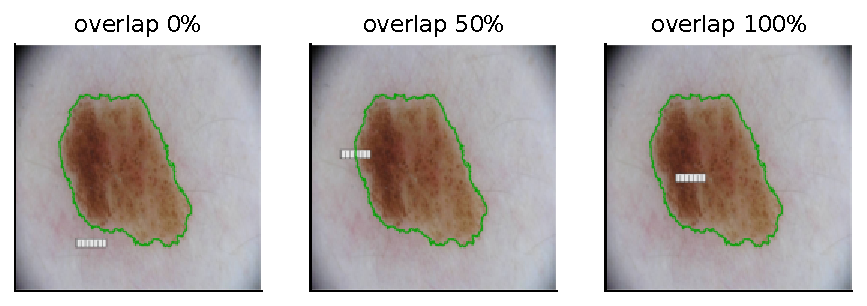
\includegraphics[width=\linewidth]{../stage1_problem_pilot_protocol/figures/ruler_examples.pdf}
\caption{The controlled sweep: the same ISIC 2018 image with the synthetic ruler at 0, 50 and 100\% overlap with the
lesion (\textcolor{roigreen}{green}: manual lesion mask). ISIC images CC BY-NC 4.0.}\label{s1:fig:ruler}\end{figure}
\begin{figure}[H]\centering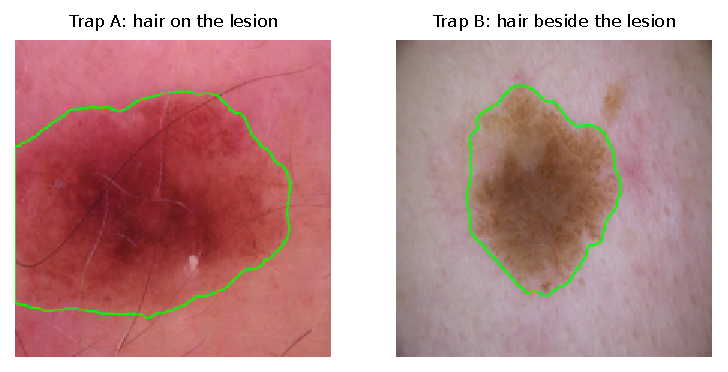
\includegraphics[width=0.78\linewidth]{../stage1_problem_pilot_protocol/figures/hair_examples.pdf}
\caption{The real hair traps (ISIC 2019): hair on the lesion (Trap~A) and beside it (Trap~B); the green line is the
lesion outline. The hair masks are not drawn because the published masks carry no licence that allows redistribution.
ISIC images CC BY-NC 4.0.}\label{s1:fig:hair}\end{figure}

\subsection{The protocol}
Table~\ref{s1:tab:protocol} lists every component with the reason it was chosen; Figure~\ref{s1:fig:env} shows the four test
environments.
\begin{table}[H]\centering\scriptsize
\caption{The protocol fixed in this stage.}\label{s1:tab:protocol}
\begin{tabular}{p{2.2cm}p{7.8cm}p{5.0cm}}\toprule
Component & Choice & Why \\\midrule
Environments & training and correlated test $P(A{=}1\mid Y{=}1)=0.9$, $P(A{=}1\mid Y{=}0)=0.1$; reversed test 0.1/0.9; clean test: no artifact (synthetic) or artifact independent of the label (real) & a strong, known shortcut whose use is exposed when the association is reversed \\
Primary metric & reversed-test AUROC; clean and correlated AUROC reported beside it & threshold-free; a model that uses the artifact must fall on the reversed test \\
Encoders & frozen DINOv2 ViT-B/14 at 518\,px (CLS token), DINOv2 at 224\,px, DermLIP (dermatology CLIP model) at 224\,px & how foundation models are used on small medical data; every arm sees the same features \\
Heads & logistic regression (liblinear, class-balanced); $C\in\{0.01,0.1,1,10\}$ and the decision threshold (maximal balanced accuracy) chosen on clean validation data only & no test or artifact information enters model selection \\
Arms & ERM; ROI masking; oracle inpainting of the artifact; group-balanced training; DFR; paired and unpaired LEACE; GroupDRO; prevalence calibration & masking is compared with methods that target the artifact itself \\
Splits & grouped by lesion identifier $\cup$ perceptual hash (Hamming $\le 8$); no group crosses a split & near-duplicates across a split inflate shortcut measurements (Sec.~\ref{s1:sec:leak}) \\
Seeds & 3 seeds (42, 123, 456) for the synthetic sweeps; 5 seeds $\times$ 5 grouped folds for the real hair traps & training and split variation are both part of the uncertainty \\
Uncertainty & crossed seed $\times$ image bootstrap, 10,000 replicates, percentile 95\% intervals & seeds share test images (Sec.~\ref{s1:sec:bootstrap}) \\
Registration & design, claims and support criteria committed to the repository before each verdict-producing run & separates confirmation from exploration \\
\bottomrule\end{tabular}
\end{table}

\begin{figure}[H]\centering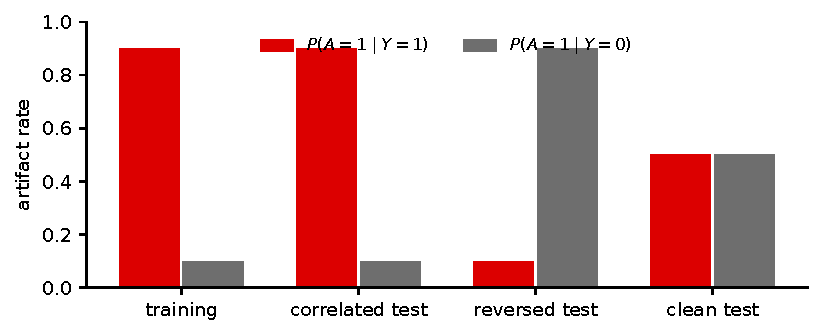
\includegraphics[width=0.78\linewidth]{../stage1_problem_pilot_protocol/figures/environments.pdf}
\caption{The trap environments. The training set and the correlated test share a strong artifact--label association;
the reversed test inverts it; the clean test removes it. A model that uses the artifact gains on the correlated test
and collapses on the reversed one.}\label{s1:fig:env}\end{figure}

\paragraph{Arms} \emph{ERM}: logistic head on the unmasked image. \emph{ROI masking}: pixels outside the lesion mask are
set to the image mean before feature extraction, at training and at test time. \emph{Oracle inpainting}: the known
artifact pixels are inpainted \citep{telea2004inpainting} --- an upper bound that needs the artifact mask.
\emph{Group-balanced}: the four artifact$\times$label cells are equally weighted. \emph{DFR}: the last layer is re-fitted
on a group-balanced subset of the validation fold \citep{kirichenko2023dfr}. \emph{LEACE}: closed-form linear erasure of
the artifact concept \citep{belrose2023leace}, either \emph{paired} (original versus artifact-removed versions of the
same images) or \emph{unpaired} (image-level artifact labels). \emph{GroupDRO} \citep{sagawa2020groupdro}.
\emph{Prevalence calibration} \citep{kina2026prevalence}. Balanced training, DFR, GroupDRO and unpaired LEACE need
image-level artifact labels; inpainting and paired LEACE need artifact masks; masking needs only the lesion mask.

\subsubsection{Leakage: grouped versus random splits}\label{s1:sec:leak}
Near-duplicate photographs of one lesion are common in ISIC. If one copy is in training and another in test, the test
measures memorisation. Every split therefore groups images by lesion identifier and perceptual hash (64-bit pHash,
Hamming distance $\le8$) and checks that no group crosses a split. To measure what this protects against, the
controlled sweep was repeated with five random image-level splits, everything else fixed.
\paragraph{Result} Random splits leave near-duplicate images on both sides of the split and inflate the measured ERM shortcut gap by 18\% (no overlap) and 10\% (full overlap), and shift both masking effects (Table~\ref{s1:tab:leak}); every analysis therefore uses grouped splits.%

\begin{table}[H]\centering\small
\caption{Leakage: grouped versus random image-level splits (controlled sweep, DINOv2@518).}\label{s1:tab:leak}
\resizebox{\linewidth}{!}{\begin{tabular}{lcccc}\toprule
Overlap & Split & Near-duplicate pairs across split & ERM gap (corr $-$ rev) & mask $-$ ERM (rev) \\\midrule
0\% & grouped & 0 & 0.241 & $+0.184$ \\
 & random (mean of 5) & 93 & 0.284 & $+0.223$ \\
100\% & grouped & 0 & 0.421 & $-0.129$ \\
 & random (mean of 5) & 93 & 0.465 & $-0.088$ \\
\bottomrule\end{tabular}}
\end{table}


\subsubsection{Uncertainty: the corrected (crossed) bootstrap}\label{s1:sec:bootstrap}
Every comparison is a paired difference in AUROC between two arms on the same test images, averaged over training
seeds (or cross-validation folds). The pilot's estimator resampled the seeds and then, \emph{independently within each
sampled seed}, the test images. In these designs, however, every seed scores the \emph{same} test images: the
controlled sweep uses one fixed test split, and in the hair traps the pooled cross-validation folds of every seed cover
the same image pool. Resampling the images independently per seed then treats one test set as several and divides the
test-sampling variance by the number of seeds, so the intervals are too narrow.
\paragraph{Why it matters} With three seeds and one test set, the per-seed estimator behaves as if the test set were
three times larger than it is. The problem is not specific to this project: any study that averages several training
seeds on one test set and resamples the images per seed has it.
\paragraph{The crossed estimator} Each replicate resamples the seeds with replacement and draws one Poisson(1) weight
per test \emph{image}, shared by every seed (and both arms) in which that image appears; the per-seed statistic is
recomputed with those weights and averaged (\texttt{wtss.stats\_crossed}; 10,000 replicates; percentile intervals).
The image weights make the test-set variance count once, as it should; the seed resampling keeps the training
variance. The estimator was registered before any interval was recomputed (\sOneRegCrossed; applied everywhere under
\sOneRegFinal).
\paragraph{Consequences for the pilot} On the \sOneCorrRows{} pilot intervals that both estimators can compute, the
crossed interval is wider by a median factor of \sOneCorrMedian{} (interquartile range \sOneCorrQlo--\sOneCorrQhi;
Figure~\ref{s1:fig:width}, Table~\ref{s1:tab:estcheck}). \sOneCorrLost{} intervals that excluded zero with the pilot's
estimator no longer do, and \sOneCorrGained{} now excludes zero (Table~\ref{s1:tab:estchanges}). Point estimates are
identical: only the uncertainty changed.
\begin{figure}[H]\centering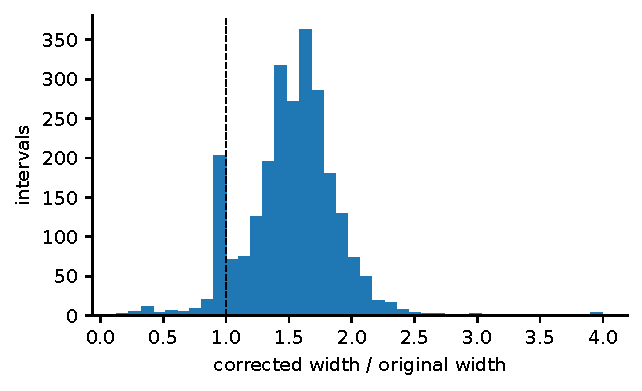
\includegraphics[width=0.58\linewidth]{../stage1_problem_pilot_protocol/figures/width_ratio.pdf}
\caption{Width of the crossed interval divided by the width of the pilot's per-seed interval, for every pilot
contrast (same predictions).}\label{s1:fig:width}\end{figure}
\begin{table}[H]\centering\scriptsize
\caption{The pilot's analyses under both interval estimators (same predictions, same point estimates; 10,000 replicates each). Width ratio $>1$: the crossed interval is wider.}\label{s1:tab:estcheck}
\begin{tabular}{p{5.0cm}p{1.4cm}p{2.6cm}p{2.6cm}p{2.4cm}}\toprule
Result group & Intervals & Excluded 0 only with the per-seed estimator & Excluded 0 only with the crossed estimator & Median width ratio (crossed / per-seed) \\\midrule
analysis/\allowbreak{}E14\_area\_ratio & 4 & 0 & 0 & 1.63 \\
spec\_e13/\allowbreak{}dermlip224\_spec & 29 & 1 & 0 & 1.45 \\
spec\_e13/\allowbreak{}dino518\_e12\_contrast & 3 & 0 & 0 & 1.44 \\
spec\_e13/\allowbreak{}dino518\_spec & 28 & 0 & 1 & 1.54 \\
synthetic/\allowbreak{}isic2018 & 114 & 6 & 0 & 1.44 \\
\textbf{all} & 178 & 7 & 1 & 1.45 \\
\bottomrule\end{tabular}
\end{table}

\begin{table}[H]\centering\scriptsize
\caption{The pilot contrasts whose verdict (interval excludes 0 or not) depends on the estimator. Every other contrast keeps its verdict.}\label{s1:tab:estchanges}
\begin{tabular}{p{4.2cm}p{5.2cm}p{3.3cm}p{2.6cm}}\toprule
Result & Contrast & Crossed estimate [95\% CI] & Verdict vs per-seed estimator \\\midrule
synthetic/\allowbreak{}isic2018/\allowbreak{}dino518\_ruler\_fixed\_corr\_main & 0.25 /\allowbreak{} mask /\allowbreak{} erm /\allowbreak{} test\_rev & $-0.059$ [$-0.127, +0.008$] & no longer excludes 0 \\
synthetic/\allowbreak{}isic2018/\allowbreak{}dino518\_ruler\_fixed\_occlusion\_occlusion & 0.0 /\allowbreak{} mask /\allowbreak{} erm /\allowbreak{} test\_uncorr & $+0.036$ [$-0.016, +0.086$] & no longer excludes 0 \\
synthetic/\allowbreak{}isic2018/\allowbreak{}dino518\_ruler\_fixed\_occlusion\_occlusion & 0.5 /\allowbreak{} mask /\allowbreak{} erm /\allowbreak{} test\_uncorr & $+0.041$ [$-0.010, +0.090$] & no longer excludes 0 \\
synthetic/\allowbreak{}isic2018/\allowbreak{}dino518\_ruler\_fixed\_occlusion\_occlusion & 0.75 /\allowbreak{} mask /\allowbreak{} erm /\allowbreak{} test\_uncorr & $+0.037$ [$-0.013, +0.086$] & no longer excludes 0 \\
synthetic/\allowbreak{}isic2018/\allowbreak{}dino518\_ruler\_fixed\_occlusion\_occlusion & 1.0 /\allowbreak{} mask /\allowbreak{} erm /\allowbreak{} test\_uncorr & $+0.039$ [$-0.010, +0.091$] & no longer excludes 0 \\
synthetic/\allowbreak{}isic2018/\allowbreak{}dino224\_ruler\_fixed\_corr\_main & 0.25 /\allowbreak{} mask /\allowbreak{} erm /\allowbreak{} test\_rev & $-0.049$ [$-0.117, +0.018$] & no longer excludes 0 \\
spec\_e13/\allowbreak{}dino518\_spec & trapA /\allowbreak{} mask /\allowbreak{} clean /\allowbreak{} all /\allowbreak{} mask /\allowbreak{} erm & $-0.023$ [$-0.045, -0.001$] & now excludes 0 \\
spec\_e13/\allowbreak{}dermlip224\_spec & trapB /\allowbreak{} leace\_unpaired /\allowbreak{} clean /\allowbreak{} all /\allowbreak{} leace\_unpaired /\allowbreak{} erm & $-0.019$ [$-0.046, +0.007$] & no longer excludes 0 \\
\bottomrule\end{tabular}
\end{table}


\subsubsection{Pre-registration}
Before every verdict-producing experiment, a document stating the design, the claims and what counts as support is
committed to the repository; results are committed afterwards, and a claim is reported whichever way it goes. The
pilot itself preceded this rule; its written specification (\texttt{docs/REPLICATION\_SPEC.md}, first commit
\sOneRegRep) serves as its registration for the replication. \textbf{Caveat:} commit times are set by the machine that
makes the commit and are not independent proof of order; registrations that are also pushed to GitHub before running
carry GitHub's time stamp as an external reference.

\subsection{The pilot and its re-implementation}
\subsubsection{What the pilot tested}
\posthoc{the pilot preceded pre-registration; its specification was written down afterwards and re-implemented}.
Table~\ref{s1:tab:pilot} lists the fifteen experiments. The pilot made five claims: (i) masking removes an artifact that
lies outside the lesion and makes the model worse than doing nothing when it lies inside; (ii) the harm is governed by
how much of the artifact survives the mask (retention), not by occlusion or lost context; (iii) methods that need
only an image-level artifact label (balanced training, DFR) fix both cases; (iv) linear erasure is insufficient for
real artifacts under the sound (paired) protocol; (v) all of this holds for real hair with pre-registered criteria on
two encoders.
\begin{table}[H]\centering\small
\caption{The pilot experiments (specification: \texttt{docs/REPLICATION\_SPEC.md}).}\label{s1:tab:pilot}
\begin{tabular}{lp{13cm}}\toprule
Exp. & What it tests \\\midrule
E1 & controlled ruler sweep, DINOv2@518: mask $-$ ERM at 0--100\% overlap; location interaction \\
E2 & the same at 224\,px (DINOv2) and with the dermatology model DermLIP \\
E3 & appearance randomisation (colour, opacity, ticks, scale of the ruler) \\
E4 & occlusion control: ruler present but uncorrelated with the label (50/50) \\
E5 & mask dilation: restoring ruler pixels around the lesion (retention) \\
E6 & same-head counterfactual sensitivity $|\Delta p|$ to inserting the ruler \\
E7 & lesion-size strata (artifact-to-lesion area ratio) \\
E8 & oracle inpainting and a prediction-consistency repair \\
E9 & bridge: group-balanced training, DFR, GroupDRO, paired LEACE at 100\% overlap \\
E10 & hair decodability from the embedding; paired LEACE on real hair \\
E11 & atlas of real artifacts (hair, ink, vignetting) in ISIC 2019 / HAM10000; vignetting trap \\
E12 & overlap-contrast trap: in-lesion versus out-of-lesion hair, no artifact-free group \\
E13 & real hair traps (Trap A in-lesion, Trap B out-of-lesion, shared hair-free group), ISIC 2019 \\
E14 & area-ratio strata of the real hair trap \\
E15 & E13 with DermLIP \\
\bottomrule\end{tabular}
\end{table}


\subsubsection{How it was re-implemented}
\registered{specification \texttt{docs/REPLICATION\_SPEC.md}, \sOneRegRep}. The pilot's code was not available for
most experiments (E9--E15), so every experiment was re-implemented from the written specification in a new code base
(\texttt{src/wtss}). A number \emph{matches} (MATCH) if it has the same sign, the same verdict on whether its interval
excludes zero, and differs by at most 0.02; SIGN+CI if sign and verdict agree but the difference is larger; MISMATCH
otherwise. Where the specification was silent or impossible to follow, the choice made is recorded with its reason
(Table~\ref{s1:tab:dev}). Two choices matter most: the hair-free group was defined as at most 30 hair pixels in the native
mask --- the only threshold that reproduces the pilot's outcome-free cell counts --- and, on the full ISIC 2019
cohort, pHash distance $\le8$ chains unrelated lesions into one giant component, so the real-hair traps apply it within
each trap pool, as the pilot's counts imply.
\begin{table}[H]\centering\scriptsize
\caption{Where the re-implementation deviates from the pilot's written specification, and why.}\label{s1:tab:dev}
\begin{tabular}{lp{3.0cm}p{4.6cm}p{7.0cm}}\toprule
\# & Specification & Re-implementation & Reason and effect \\\midrule
1 & GPU V100 32 GB & RTX 3090 24 GB & Frozen features; per-seed AUROCs of the rerun match the archive within 0.0005 (E1, E8, E9). \\
2 & Feature extraction per (seed, env) & per *view* (image $\times$ method $\times$ overlap), environments assembled by indexing & Mathematically identical (presence is a function of image/label/seed/env only); $\sim$10$\times$ fewer backbone passes. \\
3 & pHash $\le$ 8 on the full ISIC 2019 cohort (repo-default analysis) & spec E13 run: pHash $\le$ 8 within each matched trap pool (as the spec's counts imply); exploratory runs: lesion\_id $\cup$ pHash $\le$ 2 on all 25,331 & On all 25,331 images pHash $\le$ 8 chains unrelated lesions into one component of 10,974 images (same-lesion precision at distance 8: 2\%). \\
4 & Hair-free A = 0 group (threshold not stated in spec) & $\le$ 30 hair/ruler pixels in the native-resolution archive mask & Calibrated on outcome-free counts only: reproduces A0\_Y0 709 (spec 708), A0\_Y1 157 (157) and all six source proportions to 3 decimals. \\
5 & Archive mask file names & matched on zero-padded numeric id & Archive names are irregular (\_downsampled\_mvig, \_downsam\_inkmark, typos, truncated ids). 24 truncated ink ids flag their 10 candidate images as ink-uncertain (exploratory runs only). \\
6 & Images without HAM/BCN lesion\_id & source = MSK & Spec lists three sources; ISIC 2019's non-HAM/BCN images are MSK (incl. \_downsampled). \\
7 & U-Net (Ronneberger 64--1024, Task 1 only) & same architecture (+BatchNorm), 256 px, 40 epochs, Adam 1e-4, BCE+Dice, 20\% held-out pHash groups & Training hyper-parameters are not in the spec. \\
8 & Derm1M from archive & fresh clone of the official repo & Archived copy lacks bpe\_simple\_vocab\_16e6.txt.gz (.gz files were not archived); DermLIP cannot load without it. \\
9 & §3.1 "leakage inflated the gap by 27\%" & not reproduced from the archive & Pre-correction pilot used the identical split; matched-resolution gap ratio 0.96--0.97. A controlled leakage experiment is run instead (scripts/run\_leakage\_experiment.py). \\
\bottomrule\end{tabular}
\end{table}


\subsection{Results}
\subsubsection{Replication overview}
Of the \sOneNewN{} numbers the pilot reported, \sOneNewMatch{} MATCH, \sOneNewSignCI{} agree in sign and
significance but differ by more than 0.02, and \sOneNewMismatch{} MISMATCH (Table~\ref{s1:tab:ledger}). Before the
interval estimator was corrected the ledger read \sOneOrigMatch{} / \sOneOrigSignCI{} / \sOneOrigMismatch{} of
\sOneOrigN; the difference is entirely due to the wider intervals (Section~\ref{s1:sec:mismatch}).
{\scriptsize
\begin{longtable}{llp{1.7cm}p{3.3cm}l}
\caption{Replication ledger: every number the pilot reported, its re-derived value with the crossed 95\% interval, and the verdict. The pilot's own intervals came from the per-seed estimator (Sec.~\ref{s1:sec:bootstrap}) and are not reproduced; only its point values are shown.}\label{s1:tab:ledger}\\\toprule
Exp. & Quantity & Pilot (point) & Replication (crossed CI) & Verdict \\\midrule
\endfirsthead
\toprule Exp. & Quantity & Pilot (point) & Replication (crossed CI) & Verdict \\\midrule
\endhead
\bottomrule
\endlastfoot
E1 & mask $-$ ERM rev @0\% & +0.184 & +0.184 [+0.117, +0.250] & MATCH \\
E1 & mask $-$ ERM rev @25\% & -0.058 & -0.059 [-0.127, +0.008] & MISMATCH \\
E1 & mask $-$ ERM rev @50\% & -0.097 & -0.097 [-0.164, -0.030] & MATCH \\
E1 & mask $-$ ERM rev @75\% & -0.111 & -0.111 [-0.181, -0.043] & MATCH \\
E1 & mask $-$ ERM rev @100\% & -0.128 & -0.129 [-0.195, -0.064] & MATCH \\
E1 & interaction 0\% $-$ 100\% (mask) & +0.312 & +0.313 [+0.258, +0.370] & MATCH \\
E2 & dino224 mask $-$ ERM @0\% & +0.364 & +0.361 [+0.275, +0.444] & MATCH \\
E2 & dino224 mask $-$ ERM @25\% & -0.040 & -0.049 [-0.117, +0.018] & MATCH \\
E2 & dino224 mask $-$ ERM @50\% & -0.076 & -0.081 [-0.143, -0.019] & MATCH \\
E2 & dino224 mask $-$ ERM @75\% & -0.102 & -0.106 [-0.166, -0.044] & MATCH \\
E2 & dino224 mask $-$ ERM @100\% & -0.092 & -0.095 [-0.156, -0.035] & MATCH \\
E2 & dermlip224 mask $-$ ERM @0\% & +0.160 & +0.161 [+0.102, +0.222] & MATCH \\
E2 & dermlip224 mask $-$ ERM @25\% & -0.291 & -0.289 [-0.366, -0.215] & MATCH \\
E2 & dermlip224 mask $-$ ERM @50\% & -0.300 & -0.298 [-0.371, -0.225] & MATCH \\
E2 & dermlip224 mask $-$ ERM @75\% & -0.313 & -0.309 [-0.378, -0.239] & MATCH \\
E2 & dermlip224 mask $-$ ERM @100\% & -0.268 & -0.263 [-0.348, -0.180] & MATCH \\
E3 & variable ruler mask $-$ ERM @0\% & +0.147 & +0.146 [+0.082, +0.211] & MATCH \\
E3 & variable ruler mask $-$ ERM @50\% & -0.094 & -0.094 [-0.168, -0.021] & MATCH \\
E3 & variable ruler mask $-$ ERM @100\% & -0.155 & -0.155 [-0.228, -0.084] & MATCH \\
E3 & variable ruler balanced $-$ ERM @0\% & +0.103 & +0.102 [+0.068, +0.140] & MATCH \\
E3 & variable ruler balanced $-$ ERM @50\% & +0.171 & +0.171 [+0.132, +0.213] & MATCH \\
E3 & variable ruler balanced $-$ ERM @100\% & +0.222 & +0.222 [+0.181, +0.265] & MATCH \\
E4 & occlusion (50/50) mask $-$ ERM @0\% & +0.035 & +0.036 [-0.016, +0.086] & MISMATCH \\
E4 & occlusion (50/50) mask $-$ ERM @50\% & +0.033 & +0.041 [-0.010, +0.090] & MATCH \\
E4 & occlusion (50/50) mask $-$ ERM @100\% & +0.039 & +0.039 [-0.010, +0.091] & MISMATCH \\
E5 & dilate0 $-$ ERM @50\% & -0.097 & -0.097 [-0.164, -0.031] & MATCH \\
E5 & dilate10 $-$ ERM @50\% & -0.138 & -0.138 [-0.203, -0.074] & MATCH \\
E5 & dilate25 $-$ ERM @50\% & -0.153 & -0.153 [-0.221, -0.089] & MATCH \\
E5 & dilate50 $-$ ERM @50\% & -0.142 & -0.142 [-0.206, -0.083] & MATCH \\
E5 & dilate0 $-$ ERM @100\% & -0.128 & -0.129 [-0.195, -0.066] & MATCH \\
E5 & dilate10 $-$ ERM @100\% & -0.143 & -0.144 [-0.206, -0.082] & MATCH \\
E5 & dilate25 $-$ ERM @100\% & -0.144 & -0.144 [-0.209, -0.082] & MATCH \\
E5 & dilate50 $-$ ERM @100\% & -0.138 & -0.138 [-0.200, -0.082] & MATCH \\
E6 & $|\Delta p|$ erm @100\% & +0.235 & +0.235 & MATCH \\
E6 & $|\Delta p|$ mask @100\% & +0.490 & +0.491 & MATCH \\
E6 & $|\Delta p|$ mask @0\% & +0.000 & +0.000 & MATCH \\
E6 & $|\Delta p|$ erm @0\% & +0.128 & +0.128 & MATCH \\
E6 & $|\Delta p|$ erm @50\% & +0.195 & +0.195 & MATCH \\
E7 & mask $-$ ERM, large lesions @0\% & +0.249 & +0.249 & MATCH \\
E7 & mask $-$ ERM, medium lesions @0\% & +0.214 & +0.215 & MATCH \\
E7 & mask $-$ ERM, small lesions @0\% & +0.150 & +0.150 & MATCH \\
E7 & mask $-$ ERM, large lesions @50\% & +0.087 & +0.087 & MATCH \\
E7 & mask $-$ ERM, medium lesions @50\% & -0.129 & -0.129 & MATCH \\
E7 & mask $-$ ERM, small lesions @50\% & -0.325 & -0.326 & MATCH \\
E7 & mask $-$ ERM, large lesions @100\% & +0.064 & +0.063 & MATCH \\
E7 & mask $-$ ERM, medium lesions @100\% & -0.158 & -0.158 & MATCH \\
E7 & mask $-$ ERM, small lesions @100\% & -0.364 & -0.364 & MATCH \\
E14 & in-lesion hair median area ratio & +0.033 & +0.033 & MATCH \\
E14 & Trap A mask $-$ ERM, area-ratio tertile T1 & -0.064 & -0.057 [-0.095, -0.022] & MATCH \\
E14 & Trap A mask $-$ ERM, area-ratio tertile T2 & -0.057 & -0.046 [-0.082, -0.013] & MATCH \\
E14 & Trap A mask $-$ ERM, area-ratio tertile T3 & -0.059 & -0.037 [-0.071, -0.005] & SIGN+CI \\
E10 & hair decodability test AUROC & +0.943 & +0.943 [+0.919, +0.964] & MATCH \\
E10 & detector mean IoU & +0.220 & +0.222 & MATCH \\
E10 & detector median IoU & +0.180 & +0.184 & MATCH \\
E10 & LEACE A-decoder after erasure & +0.500 & +0.500 & MATCH \\
E10 & clean melanoma AUROC after erasure & +0.814 & +0.815 & MATCH \\
E10 & melanoma-head $|\Delta p|$ after erasure & +0.058 & +0.057 & MATCH \\
E10 & LEACE projection rank & +1.000 & +1.000 & MATCH \\
E12 & overlap-contrast trap mask $-$ ERM (spec: null) & +0.047 & -0.103 [-0.121, -0.085] & MISMATCH \\
E8/E9 & inpaint $-$ ERM @50\% & +0.211 & +0.211 [+0.175, +0.249] & MATCH \\
E8/E9 & inpaint $-$ ERM @100\% & +0.244 & +0.243 [+0.205, +0.284] & MATCH \\
E8/E9 & inpaint\_consistency $-$ ERM @50\% & +0.046 & +0.044 [-0.007, +0.092] & MATCH \\
E8/E9 & inpaint\_consistency\_lam0 $-$ ERM @50\% & +0.036 & +0.035 [-0.015, +0.086] & MATCH \\
E8/E9 & leace $-$ ERM @100\% & +0.294 & +0.294 [+0.249, +0.339] & MATCH \\
E8/E9 & balanced $-$ ERM @100\% & +0.281 & +0.281 [+0.236, +0.329] & MATCH \\
E8/E9 & dfr $-$ ERM @100\% & +0.279 & +0.279 [+0.220, +0.339] & MATCH \\
E8/E9 & groupdro $-$ ERM @100\% & +0.197 & +0.197 [+0.155, +0.240] & MATCH \\
E13 & trapA mask $-$ ERM (rev) & -0.064 & -0.049 [-0.083, -0.018] & MATCH \\
E13 & trapB mask $-$ ERM (rev) & +0.124 & +0.098 [+0.060, +0.136] & SIGN+CI \\
E13 & trapA inpaint $-$ ERM (rev) & +0.101 & +0.098 [+0.084, +0.112] & MATCH \\
E13 & trapB inpaint $-$ ERM (rev) & +0.108 & +0.100 [+0.083, +0.117] & MATCH \\
E13 & trapA balanced $-$ ERM (rev) & +0.213 & +0.213 [+0.183, +0.243] & MATCH \\
E13 & trapB balanced $-$ ERM (rev) & +0.234 & +0.204 [+0.166, +0.245] & SIGN+CI \\
E13 & trapA dfr $-$ ERM (rev) & +0.202 & +0.196 [+0.157, +0.235] & MATCH \\
E13 & trapB dfr $-$ ERM (rev) & +0.192 & +0.196 [+0.147, +0.251] & MATCH \\
E13 & trapA leace\_paired $-$ ERM (rev) & +0.058 & +0.074 [+0.062, +0.086] & MATCH \\
E13 & trapB leace\_paired $-$ ERM (rev) & +0.078 & +0.078 [+0.059, +0.097] & MATCH \\
E13 & trapA leace\_unpaired $-$ ERM (rev) & +0.316 & +0.320 [+0.280, +0.361] & MATCH \\
E13 & trapA mask $-$ ERM, HAM only & -0.030 & -0.011 [-0.064, +0.043] & MISMATCH \\
E13 & trapA mask $-$ ERM, BCN only & -0.078 & -0.067 [-0.110, -0.025] & MATCH \\
E15 & trapA mask $-$ ERM (rev) & -0.069 & -0.104 [-0.143, -0.067] & SIGN+CI \\
E15 & trapA balanced $-$ ERM (rev) & +0.126 & +0.146 [+0.122, +0.170] & MATCH \\
E15 & trapA dfr $-$ ERM (rev) & +0.114 & +0.116 [+0.090, +0.145] & MATCH \\
E15 & trapA leace\_paired $-$ ERM (rev) & +0.031 & +0.034 [+0.026, +0.042] & MATCH \\
E15 & trapA leace\_unpaired $-$ ERM (rev) & +0.192 & +0.203 [+0.165, +0.243] & MATCH \\
\end{longtable}}


\subsubsection{The controlled sweep (E1--E3, E8--E9)}
\begin{figure}[H]\centering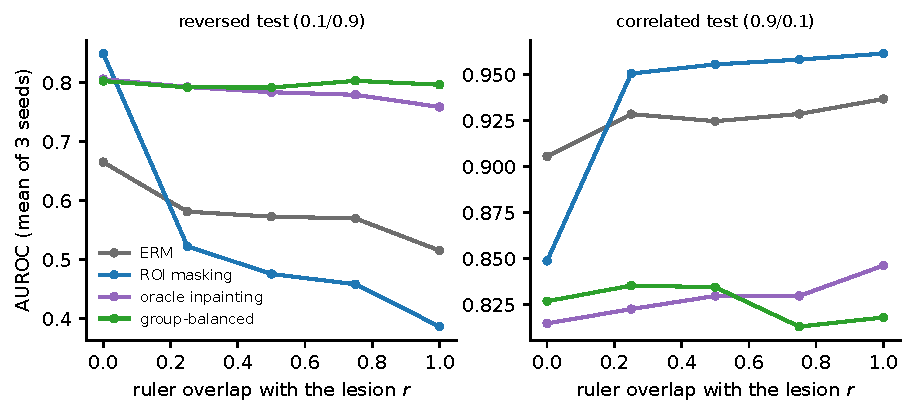
\includegraphics[width=\linewidth]{../stage1_problem_pilot_protocol/figures/pilot_sweep.pdf}
\caption{The pilot's central result, re-derived: reversed-test (left) and correlated-test (right) AUROC of four arms as
the ruler moves into the lesion (ISIC 2018, DINOv2 @518, mean of 3 seeds). Masking helps most when the ruler lies
outside the lesion and falls below ERM once it overlaps it; its correlated-test AUROC rises with overlap --- the
masked model relies on the ruler it can still see.}\label{s1:fig:pilotsweep}\end{figure}
Masking changes the reversed-test AUROC by \sOneEOneZero{} when the ruler lies outside the lesion and by
\sOneEOneHundred{} when it lies fully inside; the location interaction is \sOneEOneInter{} (Figure~\ref{s1:fig:pilotsweep}).
Two numbers show what happens. At 0\% overlap the masked model's correlated and reversed AUROC coincide
(\sOneAucmasktestcorrZeroZero{} and \sOneAucmasktestrevZeroZero): the ruler has been removed and nothing of the
shortcut remains. At 100\% overlap the masked model's correlated AUROC (\sOneAucmasktestcorrOneZero) is \emph{higher}
than ERM's (\sOneAucermtestcorrOneZero) while its reversed AUROC collapses to \sOneAucmasktestrevOneZero{} (ERM
\sOneAucermtestrevOneZero): after masking, the model uses the ruler \emph{more}.

The reversal is not a property of one encoder or one rendering. At 224\,px DINOv2 gives \sOneDinoTTFZero{} and
\sOneDinoTTFFull{} (interaction \sOneDinoTTFInter); the dermatology model DermLIP gives \sOneDermlipZero{} and
\sOneDermlipFull{} (\sOneDermlipInter); a ruler whose colour, opacity, tick pattern and scale are randomised per image
gives an interaction of \sOneStressInter.

Methods that target the artifact rather than the background all help at full overlap: oracle inpainting
\sOneSwinpaintOneZero, group balancing \sOneSwbalancedOneZero, DFR \sOneSwdfrOneZero, LEACE \sOneSwleaceOneZero{} and
GroupDRO \sOneSwgroupdroOneZero. A training-time repair that asks the model to give the same prediction with and
without the ruler (``consistency'', E8) gives \sOneSwinpaintconsistencyZeroFive{} at 50\% overlap, and \sOneSwinpaintconsistencylamZeroZeroFive{}
without its penalty ($\lambda=0$): neither is significant, and the penalty adds nothing to the augmentation.

\paragraph{The pilot's mechanism experiments (E4--E7)} replicate numerically (Table~\ref{s1:tab:ledger}): with the ruler
present but uninformative, masking does not harm (E4); dilating the mask so that more ruler pixels survive increases
the harm at 50\% overlap (E5); the masked model's prediction reacts about twice as strongly to inserting the ruler as
ERM's at full overlap (E6); and the harm is largest for small lesions (E7). What these observations imply about the
mechanism is not interpreted in this stage; only their reproducibility is.

\subsubsection{Real hair (E10, E12--E15)}
\paragraph{Cohort} Under the specification's rules the matched cells are: hair-free group \sOneCnttrapAAZeroYZero{}
benign / \sOneCnttrapAAZeroYOne{} melanoma (pilot \sOneExptrapAAZeroYZero{} / \sOneExptrapAAZeroYOne); Trap~A hair-bearing
\sOneCnttrapAAOneYZero{} / \sOneCnttrapAAOneYOne{} (pilot \sOneExptrapAAOneYZero{} / \sOneExptrapAAOneYOne); Trap~B
\sOneCnttrapBAOneYZero{} / \sOneCnttrapBAOneYOne{} (pilot \sOneExptrapBAOneYZero{} / \sOneExptrapBAOneYOne); \sOneRevMeltrapA{}
reversed-test melanomas per trap and seed, as in the pilot. The hair-free cells reproduce the pilot's counts; the
hair-bearing cells differ by 5--15\% because the lesion masks of non-HAM images come from a re-trained U-Net, which
moves some images across the overlap thresholds (a swap of mask source changes the overlap stratum of 6.9\% of
hair-bearing images and moves none from Trap~A to Trap~B).

\paragraph{E13 (DINOv2@518)} Table~\ref{s1:tab:e13dino}. Masking \emph{harms} when the hair lies on the lesion
(\sOneAdino) and helps when it lies beside it (\sOneBdino); the crossover is \sOneXdino. The masked Trap-A model still
separates the correlated test (0.917) far better than the reversed one (0.460): it uses the hair it can still see.
Every artifact-targeting arm helps in both traps; group balancing and DFR, which need only image-level hair labels,
help most (C4). Paired LEACE recovers about a third of the balanced gain (C5). Unpaired LEACE ``helps'' by
\emph{flipping} the shortcut --- its correlated AUROC (0.624) falls far below its reversed one (0.830) --- which is why
the pilot rejected it as unsound. The harm is concentrated in BCN images (\sOneSrcdinoBCN; HAM \sOneSrcdinoHAM).
Masking also costs clean-test AUROC in Trap~A (\sOneACleandino).
\begin{table}[H]\centering\scriptsize
\caption{Real hair traps (DINOv2@518; E13): AUROC in the three test environments (mean over 5 seeds) and change in reversed-test AUROC versus ERM (crossed 95\% CI). Trap A: hair on the lesion; Trap B: hair beside it; both share the hair-free group.}\label{s1:tab:e13dino}
\resizebox{\linewidth}{!}{\begin{tabular}{p{3.2cm}cccc}\toprule
Arm & Trap A: clean / corr / rev & Trap A: $\Delta$ rev vs ERM & Trap B: clean / corr / rev & Trap B: $\Delta$ rev vs ERM \\\midrule
ERM & 0.734 / 0.920 / 0.510 & --- & 0.716 / 0.894 / 0.510 & --- \\
ROI masking & 0.712 / 0.917 / 0.460 & $-0.049$ [$-0.083, -0.018$] & 0.701 / 0.795 / 0.608 & $+0.098$ [$+0.060, +0.136$] \\
oracle inpainting of hair & 0.766 / 0.906 / 0.607 & $+0.098$ [$+0.084, +0.112$] & 0.738 / 0.865 / 0.610 & $+0.100$ [$+0.083, +0.117$] \\
group-balanced & 0.785 / 0.850 / 0.722 & $+0.213$ [$+0.183, +0.243$] & 0.752 / 0.800 / 0.714 & $+0.204$ [$+0.166, +0.245$] \\
DFR & 0.715 / 0.740 / 0.705 & $+0.196$ [$+0.157, +0.235$] & 0.683 / 0.669 / 0.706 & $+0.196$ [$+0.147, +0.251$] \\
paired LEACE & 0.762 / 0.913 / 0.584 & $+0.074$ [$+0.062, +0.086$] & 0.737 / 0.876 / 0.588 & $+0.078$ [$+0.059, +0.097$] \\
unpaired LEACE (image-level $A$) & 0.726 / 0.624 / 0.830 & $+0.320$ [$+0.280, +0.361$] & \na & \na \\
\bottomrule\end{tabular}}
\end{table}

\paragraph{E15 (DermLIP@224)} Table~\ref{s1:tab:e13dermlip}. Masking harms in Trap~A (\sOneAdermlip) as the pilot
reported, but --- a finding the pilot did not test --- it harms in Trap~B as well (\sOneBdermlip), so DermLIP shows no
crossover (\sOneXdermlip). With DermLIP, removing the background costs disease signal wherever the hair lies (clean
AUROC \sOneACleandermlip{} in Trap~A).
\begin{table}[H]\centering\scriptsize
\caption{Real hair traps (DermLIP@224; E13/E15): AUROC in the three test environments (mean over 5 seeds) and change in reversed-test AUROC versus ERM (crossed 95\% CI). Trap A: hair on the lesion; Trap B: hair beside it; both share the hair-free group.}\label{s1:tab:e13dermlip}
\resizebox{\linewidth}{!}{\begin{tabular}{p{3.2cm}cccc}\toprule
Arm & Trap A: clean / corr / rev & Trap A: $\Delta$ rev vs ERM & Trap B: clean / corr / rev & Trap B: $\Delta$ rev vs ERM \\\midrule
ERM & 0.801 / 0.917 / 0.665 & --- & \na & \na \\
ROI masking & 0.735 / 0.884 / 0.561 & $-0.104$ [$-0.143, -0.067$] & \na & \na \\
oracle inpainting of hair & \na & \na & \na & \na \\
group-balanced & 0.836 / 0.875 / 0.811 & $+0.146$ [$+0.122, +0.170$] & \na & \na \\
DFR & 0.802 / 0.835 / 0.782 & $+0.116$ [$+0.090, +0.145$] & \na & \na \\
paired LEACE & 0.814 / 0.917 / 0.699 & $+0.034$ [$+0.026, +0.042$] & \na & \na \\
unpaired LEACE (image-level $A$) & 0.756 / 0.648 / 0.868 & $+0.203$ [$+0.165, +0.243$] & \na & \na \\
\bottomrule\end{tabular}}
\end{table}

\paragraph{E10: is hair visible to the encoder?} A linear probe decodes hair presence from the DINOv2 embedding with
AUROC \sOneHairDec{} ($n=\sOneHairDecN$ test images); in that set hair is \emph{less} common on melanomas
(\sOneHairPMel) than on benign lesions (\sOneHairPBen). Paired LEACE on \sOneLeaceN{} images with manual hair masks
(\sOneLeaceTrain{} training pairs) needs only one direction: the hair decoder falls from \sOneLeaceDecRaw{} to chance
(\sOneLeaceDecAfter), clean melanoma AUROC is unchanged (\sOneLeaceCleanRaw{} to \sOneLeaceCleanAfter), yet the
melanoma head's reaction to hair only falls from \sOneLeaceDpRaw{} to \sOneLeaceDpAfter. A classical morphological
hair detector (DullRazor-style) is poor: mean IoU \sOneDetIoU{} (median \sOneDetIoUMed; precision \sOneDetP, recall
\sOneDetR) --- which is why the real traps use the published masks rather than a detector.
\paragraph{E14: how large is real hair relative to the lesion?} In Trap~A the in-lesion hair covers a median
\sOneEFourteenMed{} of the lesion area, similar to the synthetic ruler. Masking harms in every tertile of this ratio
(\sOneEFourteenTOne, \sOneEFourteenTTwo, \sOneEFourteenTThree); the pilot's ``same harm at every ratio'' pattern
replicates, with the smallest harm in the tertile with the most hair.

\subsubsection{E12: the overlap-contrast design}\label{s1:sec:e12}
E12 labelled hair on the lesion as $A=1$ and hair beside it as $A=0$, with no hair-free group, and the pilot reported
a null result. The re-implementation finds masking clearly harmful (\sOneEOneTwomask), while balancing
(\sOneEOneTwobalanced) and DFR (\sOneEOneTwodfr) help. This is what the design predicts whatever the truth, because
in E12 location \emph{is} the label proxy: masking removes exactly the out-of-lesion hair that defines one side of the
contrast and keeps the in-lesion hair that defines the other. The design cannot measure a location effect; E13's
two traps with a shared hair-free group can. The pilot's null E12 result is not supported, and the design is not used
further.

\subsubsection{Audit of the pilot's written claims}
Besides the numbers, the pilot's report made statements that were checked against the archived material
(\texttt{docs/THESIS\_CLAIMS\_AUDIT.md}):
\begin{itemize}[leftmargin=*]\itemsep1pt
\item \textbf{``Leakage inflated the shortcut gap by 27\%''} --- \no\ as stated. The pre-correction pilot used the
identical split; the 27\% compared runs at different resolutions. The controlled experiment of
Section~\ref{s1:sec:leak} supports the direction with a magnitude of 10--18\%.
\item \textbf{Archived numbers} --- verified: all 21 bridge intervals of the controlled sweep were recomputed from the
archived predictions to $10^{-16}$, and a re-run from raw images reproduced 252 per-seed AUROCs within 0.0005 (a GPU
precision effect).
\item \textbf{Lesion U-Net} --- the pilot's U-Net code was missing and was re-implemented. The specification's
architecture, used for the hair traps, reaches a held-out Dice of 0.89 (pilot 0.88); a ResNet-34 U-Net used for
exploratory checks reaches 0.94.
\item \textbf{Mask-source sensitivity} --- the pilot reported that about 11\% of images change overlap stratum when the
mask source is swapped; the re-implementation finds 6.9\%, and no image moves between Trap~A and Trap~B.
\item \textbf{E11 (artifact atlas and vignetting trap)} was not re-implemented: ink appears on the lesion in too few
images (the traps exclude ink), and vignetting is a frame artifact that lies outside the lesion by construction, so it
cannot inform the in-ROI question.
\end{itemize}

\subsubsection{The mismatches}\label{s1:sec:mismatch}
\begin{enumerate}[leftmargin=*]\itemsep1pt
\item \textbf{E1, masking at 25\% overlap.} The pilot's interval excluded zero; the crossed interval includes it. The
harm is significant from 50\% overlap onward.
\item \textbf{E4, occlusion control at 0\% and 100\% overlap.} The pilot reported small positive effects of masking
with the ruler present but uninformative; with the crossed estimator they are not significant. The conclusion ---
occlusion by the mask does not harm --- is unchanged.
\item \textbf{E12.} Not null (above); a structural problem of the design.
\item \textbf{E13, HAM-only stratum.} The pilot reported harm in HAM images; the replication does not
(\sOneSrcdinoHAM). The harm is carried by BCN images.
\end{enumerate}
None of these affects the pilot's central claim --- that masking reverses from helpful to harmful as the ruler moves
into the lesion --- which replicates with every encoder and ruler rendering.

\subsection{What failed or changed in this stage}
\begin{itemize}[leftmargin=*]\itemsep1pt
\item The pilot's interval estimator was too narrow whenever seeds share test images; it was replaced, and three pilot
significance claims (E1 at 25\%, E4 at 0\% and 100\%) no longer hold.
\item E12's null result and the ``27\%'' leakage figure are not supported; the HAM-only harm of E13 does not replicate.
\item DermLIP shows no hair crossover in the replication: it is harmed by masking at both hair locations.
\item The hair-bearing cells of E13 differ by 5--15\% from the pilot's because the lesion U-Net had to be re-trained.
\end{itemize}

\subsection{Anticipated questions}
\paragraph{Why re-implement instead of re-running the pilot's code?} Most of the pilot's code for E9--E15 was not in
the archive, and re-running code verifies only that it runs. Re-implementing from a written specification tests
whether the \emph{description} is sufficient to reproduce the result, which is what a reader of a paper can do.
\paragraph{Why is the reversed test the primary metric, not the clean test?} The clean test measures disease
recognition without the shortcut, so it cannot show whether a model \emph{uses} the artifact. The reversed test
penalises reliance on the artifact directly. Both are always reported, together with the correlated test, so that a
method that simply inverts the shortcut (as unpaired LEACE does) is visible.
\paragraph{Why 0.9/0.1?} It is strong enough that every encoder learns the shortcut, which is the regime where
mitigation matters, and weak enough that both classes contain artifact-free and artifact-bearing images in training.
The same values are used everywhere, so effects are comparable.
\paragraph{Why frozen encoders and linear heads?} Every arm then uses identical features; differences between arms
are caused by the input (masked or not) or the head, not by optimisation noise. It is also the common way foundation
models are deployed on small medical datasets.
\paragraph{Why choose $C$ and the threshold on clean validation data?} Choosing them on data with the shortcut would
reward the shortcut; choosing them on reversed data would leak the test condition into training.
\paragraph{Why group by perceptual hash and not by patient?} ISIC 2018 does not publish patient identifiers; lesion
identifiers and near-duplicate detection are the strongest grouping available. The leakage experiment shows that this
grouping matters (10--18\% gap inflation otherwise).
\paragraph{Why a crossed bootstrap and not simply more seeds?} More seeds reduce training variance but do not create
new test images. The quantity of interest is a difference on a finite test set; its uncertainty must include the
sampling of that set once, which is what the shared image weights do.
\paragraph{Why do the E13 cell counts differ from the pilot's?} The hair-free group reproduces exactly. The
hair-bearing cells depend on the lesion masks of non-HAM images, which come from a re-trained U-Net; images near the
0.1 and 0.5 overlap thresholds move between strata. No image moves between Trap~A and Trap~B.
\paragraph{Why does unpaired LEACE look best, and why is it rejected?} It removes the direction that separates images
with and without hair \emph{in the training data}, where hair is strongly associated with the label; that direction
contains much of the diagnosis, and the model ends up predicting the opposite of the shortcut (correlated AUROC far
below reversed). Paired LEACE compares the same image with and without hair and removes only the hair.
\paragraph{Is 2,437 images enough?} For the controlled sweep, yes: the location interaction is large relative to its
interval (\sOneEOneInter). Individual overlap cells are less precise, which is why the 25\% cell lost significance.

\subsection{Conclusion}
\textbf{Supported.} The pilot's central result replicates from its written specification: masking helps when the
ruler lies outside the lesion and harms when it overlaps it (interaction \sOneEOneInter), with two encoders, two
resolutions and a randomised ruler; with real hair on DINOv2 masking harms in-lesion and helps out-of-lesion (crossover
\sOneXdino); methods that need only an image-level artifact label fix both traps; paired linear erasure is insufficient.
\textbf{Not supported.} The pilot's null E12 result; the ``27\%'' leakage figure; significance at 25\% overlap and in
the occlusion control; harm in HAM images; a hair crossover with DermLIP. \textbf{Fixed for the rest of the work.}
Grouped splits, clean-validation model selection, pre-registration, and the crossed bootstrap.

\subsection{Questions for the supervisor}
\begin{enumerate}\itemsep1pt
\item Is the reversed-environment AUROC acceptable as the primary metric for the thesis, or should a clinical metric
(sensitivity at a fixed specificity) be primary from the start?
\item How should the thesis present the estimator correction: as a methods detail, or as a contribution in its own
right (it affects any study that averages several training seeds on one test set)?
\item Should the E12 design and its failure be reported in the thesis (as a warning about contrast designs) or only in
the appendix?
\item Is it acceptable that the pilot's registration is its written specification, committed after the pilot ran?
\end{enumerate}

